\section{A use case for \limdds}
\label{sec:very-hard-states}

\newcommand\dicke[2]{\ket{D^{#1}_{#2}}}

In this section, we describe a family of quantum circuits we call ``Hamming weight-controlled circuits,'' which can be simulated in polynomial time using \limdds.
In contrast, we provide numerical evidence that the stabilizer rank of their output states grow rapidly in the number of qubits, indicating their hardness for stabilizer-rank-based simulation methods (see \autoref{sec:preliminaries}).

Given an $n$-qubit Clifford gate $C$, we define the $2n$-qubit Hamming weight-controlled Clifford gate (or HWC gate) $U_w^C$ on computational-basis states $\ket{x}, \ket{y}$ (both $n$ qubits) as
\begin{align}
    \label{eq:hamming-weight-control-gate}
    U^C_w(\ket{x} \otimes \ket{y}) = \begin{cases}
        \ket{x} \otimes C\ket{y} & \text{if } |x|=w \\
        \ket{x} \otimes \ket{y} & \text{otherwise}
	\end{cases}
\end{align}
where $|x|$ denotes the Hamming weight of bitstring $x$.
By Hamming weight-controlled Clifford (HWC) circuits,
we denote a sequence of HWC gates applied to initial state $\left(H\ket{0}\right)^{\otimes n}\otimes \ket{0}^{\otimes n}$.
\autoref{fig:weight-controlled-stabilizer-state}~(a) shows an example.
We refer to the output state as a HWC state.
%\todo{Tim: I removed the measurement part. I think it's safe to just talk about representation}


The \limdd representing a HWC state containing $t$ HWC gates has width $t+1\leq n+1$, and therefore has $\mathcal O(n^2)$ nodes.
\autoref{fig:weight-controlled-stabilizer-state}(b) shows an example.
%(i.e., including the \limdds that one builds during simulation of the circuit) 
First, the division of length-$n$ bitstrings depending on the Hamming weight is a known construction for BDDs~\cite{bryant86}, yielding a DD for the control register whose width which cannot exceed $n+1$. %the number of Hamming weights ${n \choose 2} = O(n^2)$.
%        \todo{are there any commonalities with the Weighted controlled ... hard functions for BDDs? Can we say something about those? Tim: @Lieuwe, you mentioned something about the top-register-DD representing a `triangle'? Is it worth adding that?}
The target register consists of a series of states $C_w \ket{0}^n$, each of which is a stabilizer state because $C_w$ is a Clifford operation.
Since Pauli-\limdds can represent $n$-qubit stabilizer states with $n$ nodes (\autoref{sec:exponential-separations}), the resulting \limdd for the entire HWC state has polynomially-many nodes.
To simulate this circuit, we build a \limdd for each individual Hamming weight-controlled Clifford gate in the Clifford circuits $C_w$.
These \limdds have polynomial size and look similar ot those in \autoref{fig:weight-controlled-stabilizer-state}.

%AL: I believe the simulation result, but don't see the proof (why wouldn't the NP-hardness of matrix x vector computation play a role?)

\begin{figure}[b!th]
	\centering
	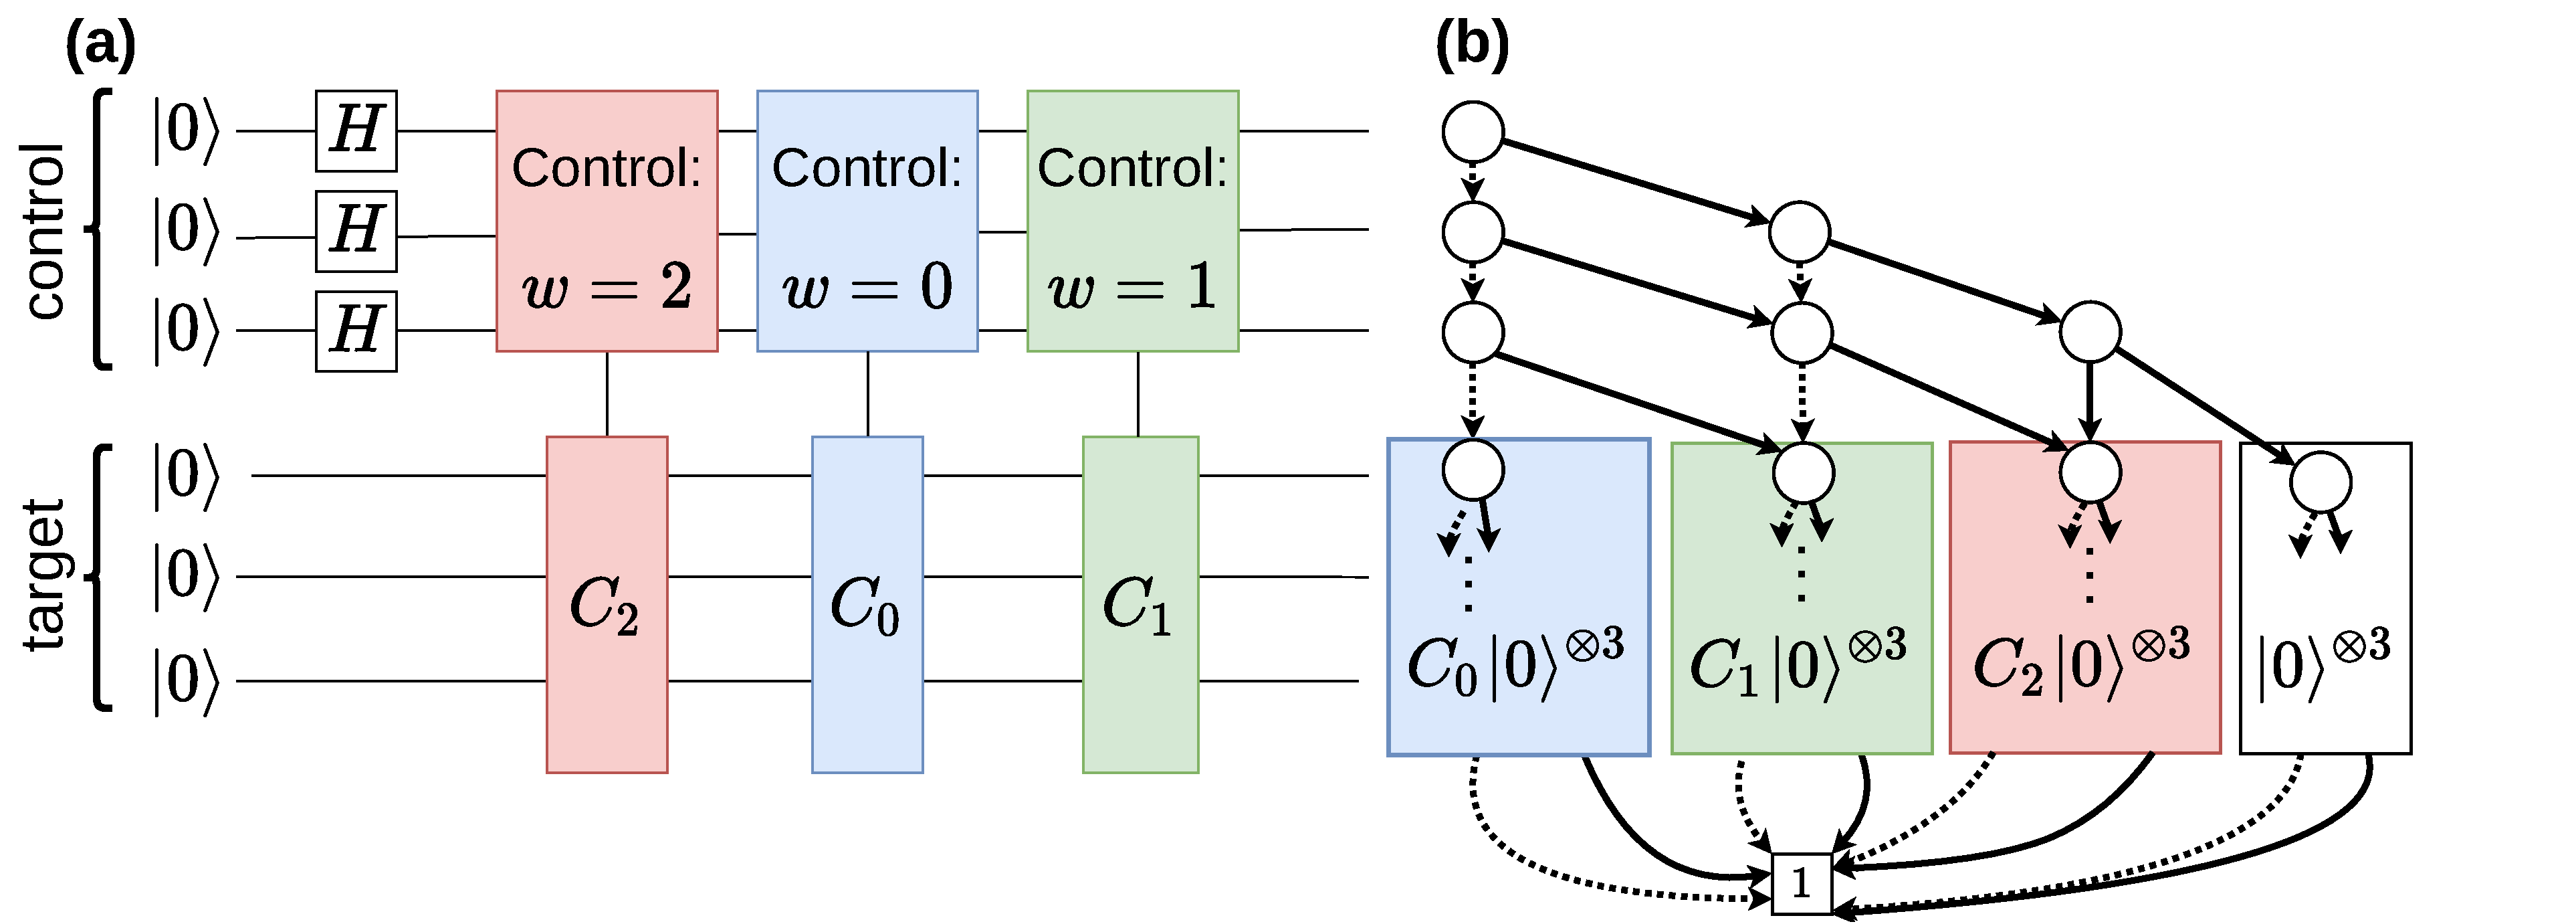
\includegraphics[width=\textwidth]{pics/weight-controlled-stabilizer-state-2.pdf}
	\caption{
        \textbf{(a)} A ``Hamming weight-controlled Clifford circuit'' on $3+3$ qubits with input state $\ket{0}^{\otimes 3} \otimes \ket{0}^{\otimes 3}$. 
        The depicted circuit consists of three controlled-Clifford gates, where the Clifford $C_w$ is only applied if the Hamming weight of the control register equals $w$ see also eq.~\eqref{eq:hamming-weight-control-gate}.
        \textbf{(b)} A Pauli-\limdd for the output state of the circuit in (a), where the colored blocks represent Pauli-\limdds for the states $C_w \ket{0}^{\otimes 3}$.
        The edges which originate in the control-register-part of the \limdd point to the top node of three different branches, each representing a constant Hamming weight of the control qubits (edge weights are all $\id$; recall dashed/solid lines represent low/high edges).
        The branch in the target-register-part corresponding to Hamming weight $w$ represents the state $C_w \ket{0}^{\otimes 3}$, which is a stabilizer state.
        We note that stabilizer states are represented by a polynomially-large \limdd (see \autoref{sec:exponential-separations}) while the width of the control-register-part of the \limdd can never exceed the possible number of Hamming weights on length-$n$ bitstrings, i.e. ${n \choose 2} = O(n^2)$.
        Consequently, Pauli-\limdds represent all Hamming weight-controlled Clifford circuits using only polynomially-many nodes.
    }
	\label{fig:weight-controlled-stabilizer-state}
\end{figure}

In order to investigate the hardness of HWC circuits for stabilizer rank methods, we employ the heuristic algorithm from \cite{bravyi2016trading} (explained in more detail in \cite{calpin2020exploring}) for searching for the stabilizer rank of Dicke states $\dicke{n}{w}$, which are equal superpositions of computational basis states with a given Hamming weight:
\[
    \dicke{n}{w} := \sum\limits_{\substack{x \in \{0, 1\}^n, \\|x| = w}} \ket{x}
    .
\]
To see that there exists HWC states $\ket{\phi}$ which have stabilizer rank $\chi(\ket{\phi})$ at least as large as the stabilizer rank $\chi(\dicke{n}{w})$of Dicke states, consider the HWC circuit consisting of the single gate $U_w^C$ where $C$ is the Pauli $X$ gate on the least significant qubit in the target register.
The resulting state is
\begin{equation}
    \label{eq:dicke}
    \ket{\phi} =
    \sum_{k=0,k\ne w}^n \dicke{n}{k}\otimes \ket{0}^{\otimes n} + \dicke{n}{w}\ket{0\ldots 01}
\end{equation}
By measuring the target register in the computational basis, the resulting control register state is $\dicke{n}{w}$ upon obtaining output $\ket{0\ldots 01}$.
Since computational-basis measurements cannot increase the stabilizer rank, we find $\chi(\ket{\phi}) \geq \chi(\dicke{n}{w})$.

\begin{table}[b!]
    \centering
    \setlength{\tabcolsep}{12pt}
    \begin{tabular}{|r|cccccc|}
        \hline
        & \multicolumn{6}{c|}{\textbf{Hamming weight $w$}}\\\hline
        \textbf{\#qubits $n$} & \textbf{0} & \textbf{1} & \textbf{2} & \textbf{3} & \textbf{4} & \textbf{5} \\\hline
        \textbf{1} & 1 &   &   &   &   &\\
        \textbf{2} & 1 & 1 &   &   &   &\\
        \textbf{3} & 1 & 2 &   &   &   &\\
        \textbf{4} & 1 & 2 & 2 &   &   &\\
        \textbf{5} & 1 & 3 & 2 &   &   &\\
        \textbf{6} & 1 & 3 & 4 & 2 &   &\\
        \textbf{7} & 1 & 4 & 7 & 4 &   &\\
        \textbf{8} & 1 & 4 & 8 & $\leq 11$  & 5 &\\
        \textbf{9} &   &   &   &   & & $>10?$  \\\hline
    \end{tabular}
    \caption{
        \label{table:stabilizer-rank-search}
        Heuristically-found upper bounds on the stabilizer rank $\chi$ of Dicke states $\dicke nw$ (eq.~\eqref{eq:dicke}) using the heuristic algorithm from Bravyi et al. \cite{bravyi2016trading} (see main text for details).
        Empty cells indicate non-existing or not-investigated states.
        In particular, we have not investigated $w> \lceil \frac{n}{2}\rceil$ since $\chi(\dicke{n}{w}) = \chi(\dicke{n}{n-w})$ because $X^{\otimes n} \dicke{n}{w} = \dicke{n}{n-w}$.
        For $\dicke{8}{3}$ and $\dicke{9}{5}$, we have run the heuristic algorithm to find sets of stabilizers up to size $11$ (theoretical upper bound) and $10$, respectively, but the algorithm has not found sets in which these two Dicke states could be decomposed.
        We emphasize that the algorithm is heuristic, so if there exists a stabilizer decomposition of a given rank, the algorithm might not find it.
    }
\end{table}

The heuristic algorithm follows a simulated-annealing approach: on input $n,w $ and $\chi$, it performs a random walk through sets of $\chi$ stabilizer states.
It starts with a random set $V$ of $\chi$ stabilizer states on $n$ qubits.
In a single `step', the algorithm picks one of these states $\ket{\psi} \in V$ at random, together with a random $n$-qubit Pauli operator $P$, and replaces the state $\ket{\psi}$ with $\ket{\psi'} := c(\id + P)\ket{\psi}$ with $c$ a normalization constant (or repeats if $\ket{\psi'} = 0$), yielding a new set $V'$.
The step is accepted with certainty if $F_V < F_{V'}$, where $F_V:= |\langle \dicke nw| \Pi_V \dicke{n}{w}|$ with $\Pi_V$ the projector on the subspace of the $n$-qubit Hilbert space spanned by the stabilizer states in $V$.
Otherwise, it is accepted with probability $\exp(-\beta (F_{V'} - F_V))$, where $\beta$ should be interpreted as the inverse temperature.
The algorithm terminates if it finds $F_V = 1$, implying that $\dicke{n}{w}$ can be written as linear combination of $V$, outputting the number $\chi$ as (upper bound to) the stabilizer rank.
For a fixed $\chi$, we use identical values to Bravyi et al. \cite{bravyi2016trading} and vary $\beta$ from $1$ to $4000$ in $100$ steps, performing $1000$ steps at each value of $\beta$.
%To determine the values of $\chi$ to investigate, we note the following two upper bounds to $\chi(\dicke{n}{w})$.
%First, following eq.~\eqref{eq:dicke}, $\dicke{n}{w}$ can be written as linear combination of ${n \choose w}$ computational-basis states so $\chi(\dicke{n}{w}) \leq {n \choose w}$.
%Second, $\dicke{n}{w} \propto \ket{0}\dicke{n-1}{w} + \ket{1}\dicke{n-1}{w-1}$, implying that we can use the sum of found upper bounds to the stabilizer ranks of $\dicke{n-1}{w}$ and $\dicke{n-1}{w-1}$ as an upper bound to $\chi(\dicke{n}{w})$.
%We ran the algorithm for $\chi$ ranging from $1$ up to the minimum of these two upper bounds.
See \cite{githubrepo} for our open-source implementation.

We provide the results of our numerical runs in \autoref{table:stabilizer-rank-search}.
Since our approach is based on using heuristic algorithms to find a good upper bound on the stabilizer rank, and not a lower bound, by construction we cannot guarantee any statement on the scaling of the rank itself.
Our approach could only have provided evidence that Dicke states do not have a rapidly scaling rank, thereby providing evidence that stabilizer-rank methods can simulate HWC states efficiently.
However, this is not what we observe, and our findings are consistent with the possibility that Dicke states have a superpolynomial rank.
Although further research is needed for a definitive answer, these numerics strengthen our confidence that \limdds can simulate HWC circuits faster than stabilizer-rank based methods.

%\section{Separation of LIMDD from known methods}
\label{sec:separation-discussion}

In the majority of this paper we have focused on the succinctness of quantum state representations in DD-based structures.
We finish off by analyzing the simulation power of Pauli-\limdds with respect to state-of-the-art quantum methods. i.e., those based on stabilizer rank~\cite{bravyi2019simulation}.
In order to establish a runtime separation, we are looking for a family of circuits that are efficiently simulatable by Pauli-\limdds, but that are not simulatable by stabilizer-rank methods or QMDDs.
For this discussion, recall that stabilizer-rank simulators require the circuits using Clifford gates only, and T-gates are implemented through gate teleportation~\cite{bravyi2019simulation}.
The resource for this are magic states, and overall efficacy of the simulation depends on the initial stabilizer rank representation of the input.

By simulation, we will mean the problem of sampling from a single chosen qubit in the Z (computational) basis, of a state generated by a quantum circuit (given as input) when applied to some simple fiducial state (e.g the all-zero state).
This is the weakest form of simulation. It should be noted however that the \limdd approach that we consider computes the final state explicitly by computing intermediate states applying gates in one by one fashion and therefore allows stronger forms of simulation.\todo{the strong form works in our favor. I mention this here} 
As additional constraint for \limdd/\qmdd, by `efficiently simulatable' we mean `produce poly-sized intermediary DDs with tractable operations'.

Our main finding is that fair comparison is difficult.
Our first example shows that, if we only allow direct simulation using stabilizer-rank simulation, it is trivial to produce circuit families where \limdds offer exponential speed-ups.
For a trivial example, consider Figure~\ref{fig:stabilizer-rank-hard}(a); if we simply consider the circuit comprising a layer of Hadamard gates, followed by a layer of $c$ T-gates, we end up in a setting where we require $\Omega(c^n)$ time for stabilizer rank-based simulators (the constant $c$ may depend on how well the n-fold product of magic states is decomposed in the stabilizer overcomplete basis, but it is widely believed that this is always exponential in $n$).
\todo{maybe replace Clifford part of circuit by hadamards?}
In contrast, the DT-\limdds perform the updates generating this state, represent and measure it efficiently. 
\todo{should argue! maybe can follow from in sec 5}

This example is of course unsatisfactory, as a quick glance reveals that, since we utilize only Z measurement(s), no tailing diagonal operators play a role in the final probabilities. In other words, the T-gate-tower can simply be ignored. 
This is a type of simple circuit rewrite which greatly extends the scope of stabilizer-rank simulator.

For a stronger example, consider replacing the T-gate tower by an interleaving of many T gates and gates which are diagonal in the computational basis.
in this case we cannot use identical arguments to simplify the circuit.
However, we can now note that any permutation matrix (w.r.t the computational basis) applied before a Z basis measurement can be executed in a post-processing step (it is just a re-labeling of the outputs). Combining this observation, with the irrelevance of diagonal operators, we see that we can ignore all permutation and phase gates before Z measurements. 

Clearly the story is more complicated if reasonable re-write and post processing rules are applied in the stabilizer-rank simulation.
Nonetheless, we have a number of examples of significantly more complex circuits, which involve linearly many T gates, even after the basic simplifications, meaning: removal of all tailing permutations and diagonal operators, and cancellation of all consecutive T-gates, within circuits.\todo{What happened to our empirical evidence? No longer relevant?}

The circuit family in Figure~\ref{fig:stabilizer-rank-hard}(b) is an example, containing many Toffoli gates~\cite{Toffoli} which each can be expressed as circuit of many T gates \todo{ref}.
It is the simplest family that we can come up that satisfying the above conditions.
As a sanity check, we proved that it is not a producing a stabilizer state.
\todo{still to do! ``Interestingly, we do this using LIMMQMDD methods (since it is not a tower IsoQMMD, this follows from canonicity in Th6 and Lemma 14). It is not simulatable by QMDD, since [add short argument]''}
We see that T gates appear in various controlled-Clifford operations, and not just in a strict layer of permutations and diagonal gates which can be resolved via post-processing we considered thus far, meaning simulation in the stabilizer rank formalism will not be efficient. 
\todo{VEDRAN: WAIT IS THIS TRUE? DOES THE BASIC REWRITE AS ABOVE NOT APPLY? PLEASE SANITY CHECK. I am worried this *again* talks about hardness of representing the state and not about hardness of output probabilities.... This is ok, but it still must be the case that we cannot apply the permutation-based and diagonal-absorption rules and get rid of all T gates that way}

One may wonder why not attempt a proof that no efficient rewrite process allows to construct equivalent efficient stabilizer-rank simulatable circuits.
This unfortunately would not be a meaningful request.
Since we consider only states which are efficiently processed by \limdd, we know there are efficient ways to simulate the circuits classically.
Consequently, if we allow \emph{all} possible rewrites, the re-write process can simply perform  \limdd-based simulation.

\todo[inline]{
Let us briefly consider the converse question of simulating stabilizer-rank-simulatable circuits in LIMQMDD.
[I DO NOT KNOW IF THE FOLLOWING IS TRUE]; Poly-sized superpositions of stabilizer states are efficiently representable in  LIMQMDD, and Clifford updates are efficient (except the Hadamard, which we perform using the mapping through the stabilizer, although other options are conceivable). 
Consequently simulation which keeps stabilizer rank low, is simulatable in our LIMQMDD as well. 
}




\begin{figure}
	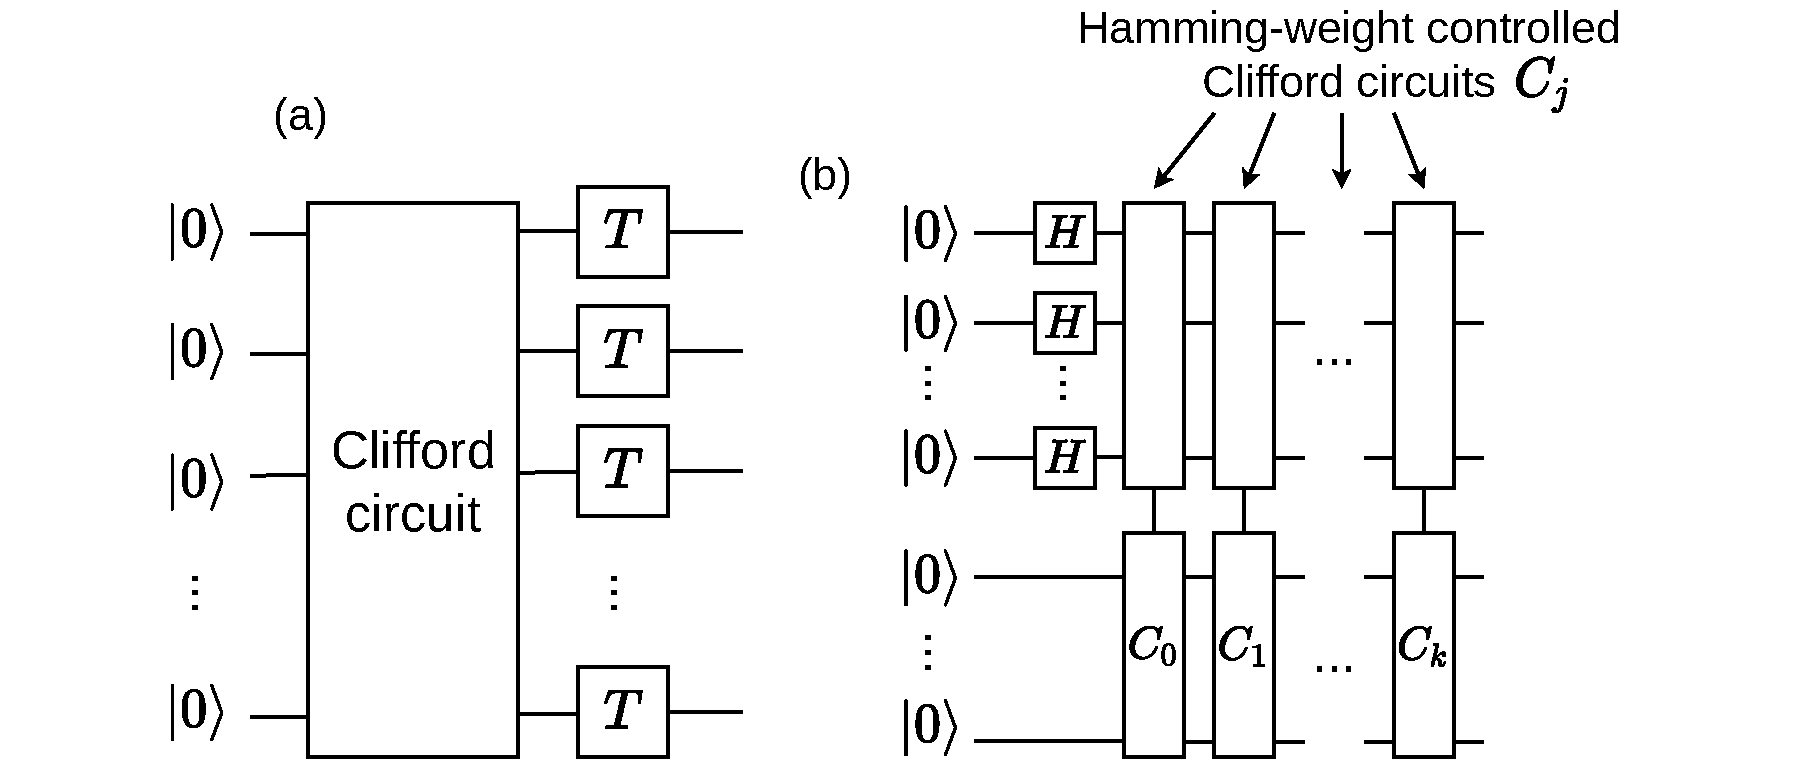
\includegraphics[width=1.0\textwidth]{pics/t-gate-tower.pdf}
	\caption{
		Circuits output a polynomially-size \limdd.
		For (b), the Hamming-weight controlled-$C$ gate on $c$ control qubits and $t$ target qubits maps $\ket{x}\otimes \ket{y}$ to $\ket{x}\otimes C\ket{y}$ if $|x| = 1$ and to $\ket{x}\otimes\ket{y}$ otherwise, for $x\in \{0, 1\}^c$ and $y\in \{0, 1\}^t$.
		Here, $|x| = \sum_{j=1}^c x_j$ denotes the Hamming weight of $x$.
		\todo[inline]{need to explain how to implement Hamming-weight controlled gate?}
		\label{fig:stabilizer-rank-hard}
	}
\end{figure}


